\section{Methodology}
    Now that the research questions have been discussed, the approach for answering those questions can be explained.
    We will start by detailing our sampling method. 
    Thereafter, we introduce the features which we think do have influence on the amount of stars that a repository has.
    Lastly, we discuss the methods for actually constructing a learning model that we can use to predict the amount of stars for a given project.
    \subsection{Sampling Method}
        When we did a first exploration of our data, we found that the distribution of stars per project is extremely right skewed: there are a lot of projects with one or zero stars, while there are much less projects which have a lot of stars, as can be seen in Figure \ref{fig:star-distribution-plot}.
        Because of this skewness, the decision was made to use so-called stratified sampling.
        With stratified sampling, we first have to divide the population into homegenous strata. 
        Thereafter, we sample an equal amount of projects from each of these strata; 
        all these samples together form the sample that is being used in the rest of the project.
        
        Each stratum has as characteristic that the amount of stars of the project in that stratum fall within a certain range. 
        The ranges that will be used in this project are: [0, 10], (10, 100], (100, 1000], (1000, +].
        Because the dataset is very large, we can also create a quite large sample:         
        out of each stratum, we will randomly select 500 projects for each stratum. The total size of our sample is thus 2000.
        
        Further, we split up our sample in a training set and a testing set. Out of our sample, we randomly pick 1000 projects which will form our training set. The remainder of the sample will be used as a testing set.
        
        Although we mentioned that the selecting of projects is completely random, it actually is not. In order to reduce bias in our sample, we decided to filter out any project by Google, Microsoft or Apple.
        The way in which they use GitHub is different from most other projects, but they do have a lot of stars, partly due to brand awareness; therefore, they are not included in our sample.
        
        \begin{figure}
            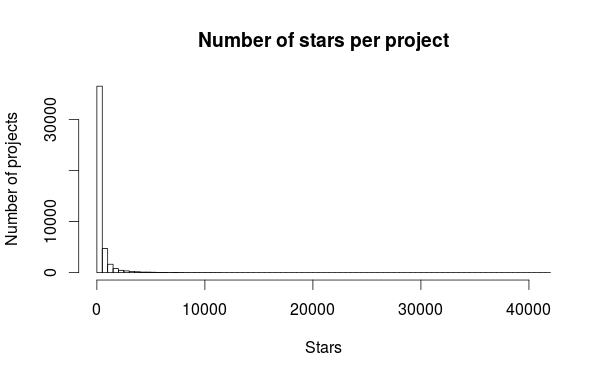
\includegraphics[width=250pt]{figures/star-distribution}
            \label{fig:star-distribution-plot}
            \caption{An histogram of the amount of stars per project}
        \end{figure}
        %\todo{
        %    \begin{itemize}
        %        \item Stratified sampling because of skewness
        %        \item Discuss strata intervals
        %        \item Discuss sample size
        %        \item Discuss items that are excluded from the sample (google/microsoft projects)
        %        \item Discuss training/testing split
        %    \end{itemize}
        %}
    
    \subsection{Features}
    In order to be able to predict the amount of stars an OSS project will get, a model need to be designed.
    Therefore a number of features is discussed first, which could influence the amount of stars on a project.
    Each of these features fall into one of the high-level groups that are specified: general project characteristics, popularity of developers or organisation, documentation and activity.
    After the features are defined, we can use them in combination with a machine learning algorithm to create the actual prediction model.

    \subsubsection{General project characteristics}
    The first group contains general features belonging to a project. 
    A feature is considered a general project feature if \todo{it cannot be categorized into the other groups}.
    In this section the different features and reasons behind choosing them will be explained.
    \begin{LaTeXdescription}
        \item[Number of commits]
        This is the total amount of commits since project creation.
        A commit can either be an addition from one of the project developers, or a merge from an accepted pull request.
        When the number of commits is larger, this might indicate that a project attracts more users.
        \item[Project country of origin]
        The country of origin refers to the country in which the project was intially created.
        This can either be based on the developer that created the project, or on the majority of developers in the organisation
        \item[Number of commits per developer]
        This is the total amount of commits that each of the developers in the project have.
        \todo{These commits do not include merge commits, so it gives an indication of the activity of each of the developers.}
        \item[Number of forks]
        The number of forks is the total amount of forks that the project got since its intial creation.
        Since forking a repository means that someone is interested and possibly want to make use of the project as a resource for their own developments, it can be a good indication of the amount of stars a project might possibly get.
        \item[Number of pull requests]
        This numerical variable contains information about how involved contributors are to the project: do they make a lot of pull requests or not?
        \item[Ratio: accepted/total pull requests]
        This numerical variable contains the number of accepted pull requests divided by the total number of pull requests. It is an indication of how `open' the project is.
        \item[Total amount of contributers]
        Someone is considered a contributer when he or she can directly commit to the repository (developer) or when a pull request is merged into the project (external-developer).
        When a project has more contributers, it might give a prediction on the amount of stars the project will possibly get.
        \item[Main programming language]
        The language that is used most throughout the project is considered the main programming language. 
        Since some languages are easier to learn and understand, projects that use that language might be able to attract more users and therefore stars.
        \item[How long does the project exists]
        Newer project might have fewer stars, since they are not discovered by the majority of the GitHub users. 
        Therefore the time a project exists, might have influence on the amount of stars the project currently has.
        \item[Number of lines of code] \todo{Larger projects have more lines of code, which can give an indication of being actively maintained or having multiple contributers -> more chance to get stars?}
    \end{LaTeXdescription}

    %name of the project
    %origin of project ('project owner'->country)
    %#commits
    %#commits/developer
    %amount of contributors on project
    %programming language
    %hoe lang bestaat het project al?

    \subsubsection{Popularity of developers or organisation}
    When a developer or organisation is already popular on GitHub, a new project created by them can get attention from other users more easily.
    This group therefore contains features that can be used to measure the popularity of a developer or organisation in order to be included in the prediction model.
    \begin{LaTeXdescription}
        \item[Average number of followers per developer]
        This is the average number of followers between all developers that contribute to the project.
        \item[Maximum number of followers per developer]
        This number indicates the maximum amount of followers the developers that contribute to the project have.
        \item[Number of developers in organisation]
        If the project is created by an organisation, this number indicates the amount of developers that belong to the organisation.
        \item[Average number of followers per developer in organisation]
        Again, if the project is created by an organisation, this number indicates the average amount of followers the developers in the organisation have.
        \item[Maximum number of followers per developer in organisation]
        This feature is like the previous one, except it now shows the maximum amount of followers a developer in the organisation has.
    \end{LaTeXdescription}

    %--Developers
    %average #followers/developer
    %max #followers/developer
    %--Organisation
    %#developers
    %average #followers/developer
    %max #followers/developer

    \todo{\subsubsection{Documentation} 
        We also think that the fact that a project is not documented very well or even not documented at all can have influence on the appreciation users show for that project. Unfortunately, this is hard to measure as some projects do have extensive documentation on their own website, while they are not using the GitHub features for documenting the project.
        At the moment of writing, it is also not possible to check if a project has a readme file or a wiki page on GitHub using the earlier discussed dataset. For future research, it might be interesting to involve this feature as well.}
    %readme present?
    %wiki files present?

    \subsubsection{Activity}
        Another thing that we think can have an impact on the amount of stars a project gets, is the activity on that project: is it actively maintained or not?
    \begin{LaTeXdescription}
        \item[Number of commits per day]
            This numerical variable measures the average number of commits per day.
        \item[Number of releases]
            Although not all projects use the releases feature of GitHub, it is interesting to see if this numerical variable does have influence.
        \item[Time between releases]
            This numerical variable is another measure of activity: it is the average time measured in days between each release for a given project.
        \item[Number of branches]         \todo{not present in dataset}
    \end{LaTeXdescription}

    %#commits/day (follow-up: issue resolution time)
    %#releases 
    %#releases/time
    %#branches

 
    \subsection{Domain}
        Since some project domains are more popular, it is easier to get stars for projects in that domain, simply because more people are interested in that domain.
        Therefore the domain is also considered in the model, to be able to make better predictions as features might weight different across domains.
        Unfortunately, the domain of a project cannot be automatically deduced from the dataset. 
        Therefore, each project in our sample was given a domain manually. Domain is obviously a categorical variable and can take the following values: \todo{decide on possible domains}.

        %\todo{
        %    \begin{itemize}
        %        \item Discuss high level features
        %        \item Specify high level features into actual metrics
        %        \item Discuss adding of the `domain' to filter popular domain areas
        %    \end{itemize}
        %}
    
    
    \subsection{Finding relations}
        Now that the features have been listed, we can try to infer relations between those features. More specifically, we have an independent variable - the amount of stars for a project - and we will try to correlate it with the independent variables - the features listed in the previous section.
        
        The machine learning algorithm that first comes to mind is linear regression. However, some of our features are categorical, e.g. the programming language of a project, which makes it impossible to use linear regression.
        Luckily, there is a variant available which is able to handle categorical variables; this algorithm is called `multiple linear regression'. 
        Initially, this algorithm will be used. Depending on the results, we will try out other algorithms like random forest and naive bayes.
        
        On top of the initial analysis using multiple linear regression, an attempt will be made to finetune our model so that the prediction is as accurate as possible. The step-wise regression algorithm will be used for this task.
    
       %\todo{
       %     \begin{itemize}
       %         \item Discuss machine learning algorithms (Multiple Linear Regression, Stepwise regression)
       %     \end{itemize}
       % }
